\documentclass[letterpaper]{article} % DO NOT CHANGE THIS
\usepackage[submission]{aaai2026}  % DO NOT CHANGE THIS
\usepackage{times}  % DO NOT CHANGE THIS
\usepackage{helvet}  % DO NOT CHANGE THIS
\usepackage{courier}  % DO NOT CHANGE THIS
\usepackage[hyphens]{url}  % DO NOT CHANGE THIS
\usepackage{graphicx} % DO NOT CHANGE THIS
\urlstyle{rm} % DO NOT CHANGE THIS
\def\UrlFont{\rm}  % DO NOT CHANGE THIS
\usepackage{natbib}  % DO NOT CHANGE THIS AND DO NOT ADD ANY OPTIONS TO IT
\usepackage{caption} % DO NOT CHANGE THIS AND DO NOT ADD ANY OPTIONS TO IT
\usepackage{amsmath}
\usepackage{amssymb}
\frenchspacing  % DO NOT CHANGE THIS
\setlength{\pdfpagewidth}{8.5in} % DO NOT CHANGE THIS
\setlength{\pdfpageheight}{11in} % DO NOT CHANGE THIS
%
% These are recommended to typeset algorithms but not required. See the subsubsection on algorithms. Remove them if you don't have algorithms in your paper.
\usepackage{algorithm}
\usepackage{algorithmic}

%
% These are are recommended to typeset listings but not required. See the subsubsection on listing. Remove this block if you don't have listings in your paper.
\usepackage{newfloat}
\usepackage{listings}
\DeclareCaptionStyle{ruled}{labelfont=normalfont,labelsep=colon,strut=off} % DO NOT CHANGE THIS
\lstset{%
	basicstyle={\footnotesize\ttfamily},% footnotesize acceptable for monospace
	numbers=left,numberstyle=\footnotesize,xleftmargin=2em,% show line numbers, remove this entire line if you don't want the numbers.
	aboveskip=0pt,belowskip=0pt,%
	showstringspaces=false,tabsize=2,breaklines=true}
\floatstyle{ruled}
\newfloat{listing}{tb}{lst}{}
\floatname{listing}{Listing}
%
% Keep the \pdfinfo as shown here. There's no need
% for you to add the /Title and /Author tags.
\pdfinfo{
/TemplateVersion (2026.1)
}

\setcounter{secnumdepth}{0} %May be changed to 1 or 2 if section numbers are desired.

% Title
\title{Interpretable Machine Learning for Predicting Adverse Drug Interactions in Singapore}
\author{
    % Authors - Replace with actual names
    An Xiao\textsuperscript{\rm 1},
    Liu Lexi\textsuperscript{\rm 2},
    Zhou Zirun\textsuperscript{\rm 3}
}
\affiliations{
    % Affiliations
    \textsuperscript{\rm 1}School of Computing, National University of Singapore\\
    student1@nus.edu.sg, student2@nus.edu.sg, student3@nus.edu.sg
}

\begin{document}

\maketitle

\begin{abstract}
The rapid advancement of healthcare systems and increased life expectancy have led to a growing prevalence of polypharmacy, particularly among elderly patients in Singapore. This paper proposes an interpretable machine learning application to predict the risk of adverse drug interactions, providing transparent explanations to support clinical decision-making tailored to the Singapore context.
\end{abstract}

\section{Introduction}

The rapid advancement of healthcare systems and increased life expectancy have led to a growing prevalence of polypharmacy, where patients—particularly elderly individuals—are prescribed multiple medications simultaneously. While such multi-drug therapies are often necessary for managing chronic conditions, they significantly increase the risk of drug-drug interactions (DDIs). Statistics show that DDIs may greatly contribute to a worsening patient condition through adverse side effects.\cite{Chan2016:chan}, and the risk of DDIs is underperceived by the medical industry.\cite{polypharmacy}

DDI is especially critical in Singapore.\cite{Ho2023} Given that there is a vacuum in reliable formal methods among Singaporean doctors to avoid drug interactions, we propose to leverage machine learning algorithms to provide explainable advice to Singaporean doctors on possible drug interactions for every prescription. We first show that drug interaction is an important issue that can be properly addressed through machine learning algorithm under Singaporean context. We will then expound on the further details in our choice of the machine learning algorithm and its training process. Last but not the least, we will demonstrate the result of our prototypical machine learning application and how it benefits Singapore's medical industry through providing explainable advice on potential drug interactions in prescriptions.


\section{Motivation}

\subsection{Drug interactions as a severe issue in Singapore}

DDI has been recognised as a significant contributor to the degeneration of patient health \cite{polypharmacy,Chan2016:chan}. The complexity of managing multiple medications increases the likelihood of unintended interactions, making it crucial for healthcare providers to have effective tools for predicting and preventing DDIs.

Singapore presents a particularly important context for addressing this problem. First, the country's demographic structure is shifting toward an ageing society, with a high proportion of elderly individuals requiring long-term medication.\cite{singstat_population_2025} Figure 1 shows our rough estimate of the elderly population in Singapore in 2025 based on the age distribution of the population and the stratified death rate of different age groups\cite{singstat_death_rate_2025} in Singapore in 2025. With aging population, the number of senior citizen is expected to proliferate in the upcoming decades, which indicates a sharp increase in the demand of polypharmacy due to the positive association between seniority of an individual to more complex medication needs.\cite{Ho2023,Wong2019} 

\begin{figure}[t]
    \centering
    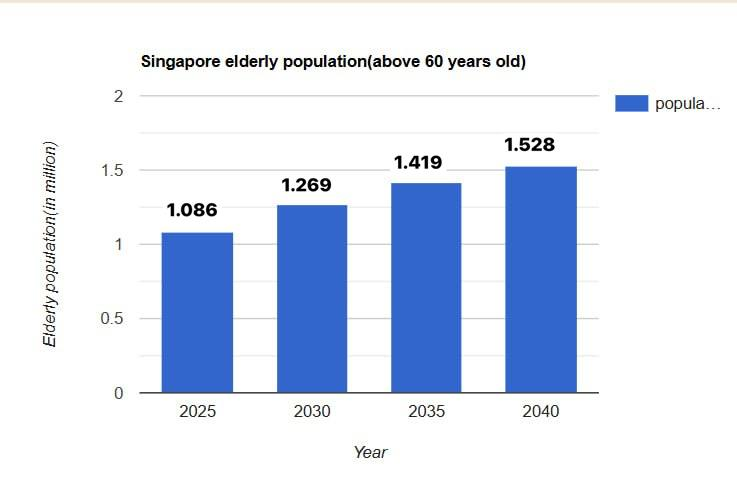
\includegraphics[width=0.95\columnwidth]{./population.png}
    \caption{Predicted elderly Population(above 60) of Singapore in 2025.}
    \label{fig:population_pyramid}
\end{figure}

Second, Singapore exhibits a unique disease profile, with high rates of metabolic and cardiovascular conditions, which often necessitate multi-drug treatment plans.\cite{hop_health_concerns_2025} 

Third, the healthcare system in Singapore emphasises precision medicine and efficient clinical decision-making, creating a strong demand for tools that can assist healthcare professionals in evaluating complex prescription combinations.Even though there are drug interaction database and alogrithms available, the data are mostly collected from a more Western profile. The bias in the data collected may lead to potential underrepresentation of certain diseases that are more common among Singaporeans. The underrepresentation indicates that the current algorithms may not be the most appropriate under Singaporean context and there is a significant space for improvement for us.  

\subsection{Why machine learning algorithms}

Machine learning has been effective in detecting patterns of drug interactions as it can be categorised as a classification task.\cite{Gheorghita2025} When the number of drugs involved in a single prescription increase, we expect the number of possible pair of drugs that may produce interaction to increase exponentially($N =$ $n\choose2$, n is the number of drugs and N is the number of possible pairs), which eventually leads to human oversight. 

We can further leverage the strengths of interpretable ML models—such as their ability to provide human-understandable decision rules and feature contributions—to ensure that medical professionals can trust and effectively utilise the model's predictions. More details will be explored in the solution section.

\subsection{Ethical considerations}

While the previous sections mention the advantages of using machine learning algorithms to detect drug interactions, we also acknowledge the important ethical considerations as the healthcare industry typically involves high-stake responsibilities where many believe that human decisions must be involved. Drug prescription is no exception. 

First, any misjudgement by the algorithm must be held accountable. The machine learning algorithm can never make any independent judgement on its own without human oversight. The patient, who are unable to judge the accuracy of the predicted drug interaction result, should also not be exposed to the decision making process. Therefore, we envision the algorithm to be most ethically positioned as advisory to the doctors, with which the doctor gives the final decision on whether the drug interaction may actually happen and be held accountable for his own judgement as a medical professional.

\section{Method}

We first define the input and the output of our machine learning model. The input is a pair of drugs and the patient's condition, and the output contains the possibility predicted about whether the two drugs interact with each other.
We mathematically express our model as follows:

\begin{equation}
    \hat{y} = F(D_A, D_B)
\end{equation}

where $D_A, D_B \in \mathbb{R}^{d}$ are the molecular fingerprints of Drug A and Drug B with dimension $d$, respectively, and $c$ is the patient's condition vector. The function $F$ represents the machine learning model that takes these inputs and produces a prediction $\hat{y}$ indicating the probability of an interaction. In our experiment, we use random forest  as our machine learning models, which will be further explained in the next section.

Then with the output possibility $\hat{y}$, we can further apply a threshold to determine whether the drug pair is predicted to interact or not. For example, if $\hat{y} > 0.3$, we can classify the drug pair as interacting; otherwise, we classify it as non-interacting. After interacting pairs are identified, we can further provide an explanation of the interaction through the interpretable machine learning model, which will be discussed in the next section.

Additionally, with the predicted interaction, we can further predict the severity of the interaction of the drug pair. For example, we can classify the severity into three levels: mild, moderate, and severe based on the patient's condition and the predicted interaction. This can be achieved by training a separate model that takes the predicted interaction and patient's condition as input and outputs the severity level.

\subsection{Input construction}

\subsubsection{Drug Interaction Pairs}
For the input, we represent each drug using its molecular fingerprint represented by MACCS keys. MACCS keys converts chemical structures into a binary vector of 166 dimensions based on the presence or absence of specific chemical substructures.\cite{rdkit} It is also widely adpoted in pharmaceutical research as a form of data representation of drugs\cite{xie2020improvement,durant2002reoptimization} The model learns to predict the interaction label based on the combined features of the two drugs.
For instance, the 120 th dimension of the input vector indicates the presence of a benzene ring.\cite{rdkit}

To combine the two drug fingerprints into a single input vector, we perform addition of the two 166-dimensional vectors, resulting in a trinary 166-dimensional vector that captures the combined chemical features of both drugs. In other words, the input vector for a drug pair is represented as:

\begin{equation}
    x_i = \begin{cases}
        0 & \text{if neither drug has the substructure} \\
        1 & \text{if exactly one drug has the substructure} \\
        2 & \text{if both drugs have the substructure} 
        \end{cases}
\end{equation}

where $x_i$ is the $i$-th dimension of the input vector, corresponding to the $i$-th MACCS key. 

This new representation resolves two major challenges. First, most machine learning algorithms only took one single vector as input, and the addition operation allows us to combine the two drug fingerprints into a single vector without losing any information. Second, the addition operation is commutative, which means that the order of the drugs does not affect the input representation. This is important because drug interactions are symmetric; if Drug A interacts with Drug B, then Drug B interacts with Drug A.

\subsubsection{Patient Condition}

A simple binary vector will be used to represent the presence or absence of certain conditions that are relevant to drug interactions. This allows the model to consider how patient-specific factors may influence the likelihood and severity of drug interactions.


\subsubsection{Data source}
\ 
\newline
We use the BIOSNAP ChChMiner dataset, which is derived from DrugBank and contains experimentally validated drug-drug interaction (DDI) pairs. Each entry in the raw dataset consists of two DrugBank IDs indicating that the pair of drugs is known to interact and should not be used together. After filtering out drug pairs for which molecular structures could not be retrieved, our dataset contains approximately 40,000 positive examples (interacting pairs). 

\subsubsection{Negative sample construction}
\ 
\newline
The BIOSNAP dataset only contains known positive interactions. Since no ground-truth negative pairs are provided, we construct negative examples by randomly sampling drug pairs that do not appear in the positive set. We follow the standard 1:1 positive-to-negative ratio.

We acknowledge that this procedure relies on the assumption that pairs absent from DrugBank are treated as non-interacting, though some may represent undiscovered interactions. This is a well-recognised limitation of DDI benchmarks and is consistent with prior work in this area.

\subsubsection{Molecular feature representation}
\ 
\newline
Each drug is represented as a 166-dimensional binary fingerprint generated using the MACCS Keys (Molecular ACCess System) scheme via RDKit. MACCS Keys encode the presence or absence of 166 predefined chemical substructures, such as the presence of a benzene ring (Key 120), a carboxyl group (Key 148), or a nitrogen-containing heterocycle (Key 80). Each bit is either 1 (substructure present) or 0 (absent).

During data preprocessing, we removed MACCS bits with zero variance across all drugs in the dataset, which also means the bits that are either universally present or universally absent. These features carry no discriminative information and their removal reduces noise in the input representation. After this filtering step, the effective fingerprint dimensionality is reduced from 166 to 162 bits per drug, resulting in a final feature vector of 324 dimensions per drug pair.

We chose MACCS Keys over the more commonly used Morgan fingerprints mainly because each MACCS bit corresponds to a named, chemically interpretable substructure, which directly supports our interpretability analysis using SHAP. 

\begin{equation}
    x = [\mathbf{fp}_A \| \mathbf{fp}_B] \in \{0,1\}^{324}
\end{equation}

\subsubsection{Symmetry augmentation}
\ 
\newline
DDI is inherently symmetric because if Drug A interacts with Drug B, then Drug B interacts with Drug A. However, the concatenation scheme above is order-sensitive: $[\mathbf{fp}_A \| \mathbf{fp}_B] \neq [\mathbf{fp}_B \| \mathbf{fp}_A]$.
To prevent the model from learning spurious positional biases, we augment the dataset by including both orderings of every drug pair, effectively doubling the dataset size.

\subsubsection{Dataset splits}
\ 
\newline
The final dataset is split into training, validation, and test sets at an 80/10/10 ratio, with stratification to preserve the class balance across all splits.

\subsection{Algorithm and models}
We train four models of increasing complexity on the same dataset and splits, so that performance differences can be attributed solely to model architecture.

\subsubsection{Logistic Regression}
\ 
\newline
Logistic Regression serves as our linear baseline. It computes a weighted sum of all 324 input features and passes the result through a sigmoid function to produce an interaction probability:

\begin{equation}
    \hat{y} = \sigma(\mathbf{w}^T \mathbf{x} + b)
\end{equation}

Despite its simplicity, logistic regression provides a meaningful lower bound on performance and highlights the limitations of linear decision boundaries in this task. 

\subsubsection{Random Forest}
\ 
\newline
Random Forest is an ensemble of decision trees, each trained on a random bootstrap sample of the training data with a random subset of features considered at each split. Predictions are aggregated by majority vote across all trees.

This model introduces two important capabilities over logistic regression. First, individual decision trees can capture non-linear feature interactions. For example, learning rules such as "if Drug A contains a CYP3A4-related motif AND Drug B contains an aromatic ring, predict interaction." Second, the ensemble mechanism reduces overfitting by averaging over diverse trees that each capture different patterns in the data. We train a forest of 100 trees with all other hyperparameters set to their sklearn defaults.

\subsubsection{MLP}
\ 
\newline
Our Multi-Layer Perceptron consists of three fully-connected hidden layers with ReLU activations and dropout regularisation:

\begin{center}
    $324 \rightarrow 256 \rightarrow 128 \rightarrow 64 \rightarrow 1$
\end{center}
Dropout with probability 0.3 is applied after each of the first two hidden layers to reduce overfitting. The output layer uses a sigmoid activation to produce an interaction probability. The model is trained with the Adam optimiser (learning rate $10^{-3}$) and binary cross-entropy loss for 50 epochs, with the best checkpoint selected based on validation AUC-ROC.

Compared to Random Forest, the MLP learns hierarchical, distributed representations of the drug pair, allowing it to capture more abstract feature interactions. However, it treats the concatenated 324-dimensional vector as a flat input, with no explicit mechanism to compare features across the two drugs.

\subsubsection{MLP with Attention}
\ 
\newline
To address the limitation above, we introduce a cross-drug attention mechanism. Instead of immediately flattening both fingerprints into a single vector, we first encode Drug A and Drug B separately through a shared encoder:

\begin{equation}
    \mathbf{h}_A = \mathrm{Encoder}(\mathbf{fp}_A), \mathbf{h}_B = \mathrm{Encoder}(\mathbf{fp}_B)
\end{equation}

\subsection{Training process}
\section{Results}
\bibliography{CS3264_Final_Report}

\end{document}
